\documentclass[10pt]{article}

\usepackage{fancyhdr}
\usepackage[includeheadfoot,left=1in, right=1in, top=0.5in, bottom=0.5in]{geometry}
\usepackage{lastpage}
\usepackage{extramarks}
\usepackage[usenames,dvipsnames]{color}
\usepackage{graphicx}
\usepackage{listings}
%\usepackage{courier}
\usepackage{float}
\usepackage{url}
\usepackage{subfigure}
\usepackage{varwidth}
\usepackage{caption}
\usepackage{multirow}
\usepackage[pdfborder={0 0 0}]{hyperref}
\usepackage[compact,small]{titlesec}
\usepackage{microtype}
\usepackage{verbatim}
\usepackage{booktabs}
\usepackage{indentfirst}
\usepackage{pgffor}
\usepackage[table]{xcolor}
\usepackage{bytefield}
\usepackage{textcomp}
\usepackage{lipsum}

%\rowcolors{2}{gray!25}{white}

\parskip = 0.5\baselineskip
\setlength{\belowcaptionskip}{-\baselineskip}

\captionsetup{font=scriptsize}
\captionsetup{labelfont=bf}

\pagestyle{fancy}
\rhead{Max Thrun}
\lhead{8-Bit Softcore CPU}
\rfoot{Page\ \thepage\ of \protect\pageref{LastPage}}
\cfoot{}
\renewcommand\headrulewidth{0.4pt}
\renewcommand\footrulewidth{0.4pt}

% make verbatim text small
\makeatletter
\g@addto@macro\@verbatim\tiny
\makeatother

\setlength\parindent{0pt} % Removes all indentation from paragraphs

\definecolor{sh_comment}{rgb}{0.12, 0.38, 0.18 } %adjusted, in Eclipse: {0.25, 0.42, 0.30 } = #3F6A4D
\definecolor{sh_keyword}{rgb}{0.37, 0.08, 0.25}  % #5F1441
\definecolor{sh_string}{rgb}{0.06, 0.10, 0.98} % #101AF9

\lstset{
    language={[x86masm]Assembler},
    xleftmargin=.25in,
    xrightmargin=.25in,
    numbers=left,
    numberstyle=\tiny,
    frame=tb,
    showstringspaces=false,
    captionpos=b,
    stringstyle=\color{sh_string},
    keywordstyle = \color{sh_keyword}\bfseries,
    commentstyle=\color{sh_comment}\itshape,
    basicstyle=\footnotesize\sffamily,
    morekeywords={.define,stl,ld,brz,ldl},
    %numbersep=-5pt,
    belowskip=\baselineskip,
    aboveskip=\baselineskip
}

\let\oldtabular\tabular
\renewcommand{\tabular}{\footnotesize\oldtabular}

\newcommand{\placementimage}[2]{
    \begin{figure}[H]
        \centering
        \includegraphics[width=\linewidth, height=4in, keepaspectratio]{#1}
        \caption{#2}
    \end{figure}
}

\newcommand{\specialcell}[2][c]{\textbf{\begin{tabular}[#1]{@{}c@{}}#2\end{tabular}}}

\title{
    \vspace{0.5in}
    \textmd{\textbf{8-Bit Softcore CPU}}\\
    \vspace{2in}
    \textmd{\textbf{Submitted as the Capstone Project for\\the Master of Engineering Degree}}\\
    \vfill
}
\author{\textbf{Max Thrun}}

\begin{document}
\clearpage\maketitle
\thispagestyle{empty}
\newpage
\section{Abstract}

The purpose of this project is to create a custom 8-bit softcore computer
processing unit (CPU) which can ultimately be used and expanded on for both
educational and practical purposes. This project explores the design and
implementation of a complete system on chip (SoC) in the hardware description
language Verilog and realized on a field programmable gate array (FPGA). A
simple assembler and program loader, written in Python, are also explored to
form a complete development package. With these components we are able to
compile programs written in our custom assembly language and run them on our
custom CPU in a FPGA development board.

\section{Introduction}

The understanding, design, and implementation of a computer processing unit is
something that is often challenging for most people when first studying the
field. There are seemingly infinite resources on the subject but there are very
few that provide a top to bottom example going from them compiler down to the
hardware.

When I personally started studying the topic of CPUs I had a strong urge to
implement my own and be able to compile and run small programs on it which is a
sentiment I feel is common amongst people first getting interested in the
topic.  Like many, I have found that I often learn best by example and I was
frustrated at the time with the lack of easy to understand example projects out
there. It was not until I came across the Your First CPU! \cite{yfcpu} blog
posts, which provided a simple concrete example of implementing a CPU, that
things really clicked. The Your First CPU!  blog posts were good at helping me
get an understanding of a CPU on the hardware level but it left a lot to be
desired on the software end as it provided fairly complex Flex and Bison
\cite{flex} scripts to parse and assemble programs. While these tools are
popular and extremely powerful I felt that they were over complicated for what
I wanted to achieve at the time which was to just simply compile a small
program and run it on my custom CPU.

There are numerous other example projects out there of CPUs but most that I
have come across in the past were either too complex, incomplete, or just
implemented in a way that I personally found confusing.  With this project I
try to bridge some of these gaps by providing a small, simple, working example
of a CPU as well as providing a basic assembler and a tool to load and run
programs.

\newpage
\section{Implementation}

    \subsection{Design Overview}

    The main goal of this project is to show an example of a working CPU. While
    this can be achieved purely through simulation it is much more satisfying
    to see a physical implementation running on a development board which can
    provide various inputs and outputs (IO).  For my implementation I chose to
    use an Altera DE-1 development board which has a Cyclone II FPGA and a
    plethora of various IO such as LEDs, switches, 7 segment displays, as well
    as more complex peripherals such as audio.

    In order to communicate with these peripherals we need additional
    components besides the CPU. Firstly, we need random access memory (RAM)
    which we will use to store our program and which the program will use to
    store information while it is running. The Cyclone II, like most modern
    FPGAs, has internal RAM which we can use for this purpose.  Secondly, we
    need some general purpose input and output (referred to as GPI and GPO in
    this project) modules in order to interface with peripherals such as LEDs
    and switches. Additionally, we would like to have some way of performing
    timed events, such as flashing the LEDs a certain rate. A 32-bit timer
    module has been implemented to achieve this. When the CPU needs to read or
    write data we need module which can determine if the CPU is trying to talk
    to RAM or a peripheral. This module is called a memory mapper as it maps
    different memory locations as seen by the CPU to various other components
    throughout the system. Finally, we need a way to load the programs into the
    system which is achieved by a serial bootloader.

    A system block diagram which illustrates the connection between the DE-1
    peripherals and the various components in the design is shown below.

    \begin{figure}[H]
        \centering
        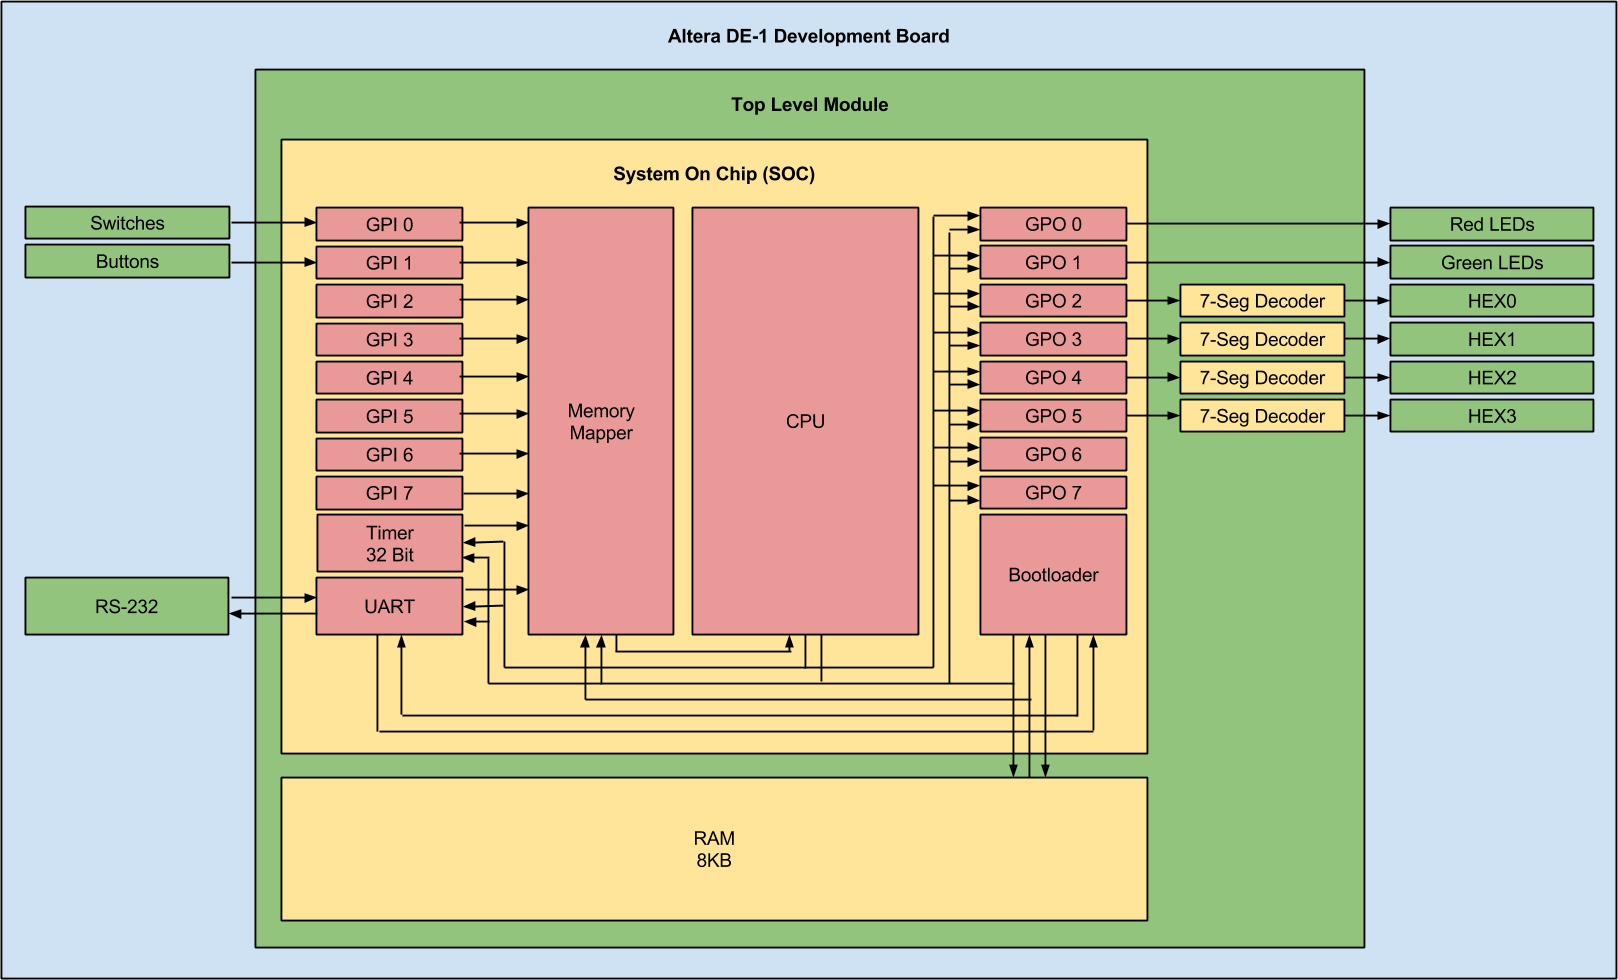
\includegraphics[width=\linewidth]{./block_diagram.png}
        \caption{System Block Diagram}
    \end{figure}



    \subsection{CPU}

        \begin{figure}[H]
            \centering
            \begin{minipage}[t]{.7\textwidth}
                \vspace{0pt}
                The CPU for this project is non-piplined and each instruction
                takes 7 clock cycles to complete.  Additionally, I have chosen
                to go with a Von Neumann style architecture \cite{von} where
                the data and instructions are both stored in the same memory
                and accessed by a single bus. The reason for this over a
                Harvard style architecture \cite{harvard} is that it is
                slightly simpler to implement and also allows us to more easily
                achieve cool tricks such as having a program modify its own
                code \cite{modify}. One of the down sides of using a Von
                Neumann architecture is that you cannot access the instruction
                and data memory at the same time. This means that you would
                typically need a whole extra cycle just to fetch or store data.
                To avoid this I am actually clocking the CPU on opposite edge
                of the clock relative to the rest of the system.  This means
                that the CPU steps on the positive edge and the memory responds
                on the negative edge which allows the data to be ready by the
                next CPU cycle. This saves us 2 clock cycles per instruction.
            \end{minipage}%
            \begin{minipage}[t]{.3\textwidth}
                \vspace{0pt}
                \centering
                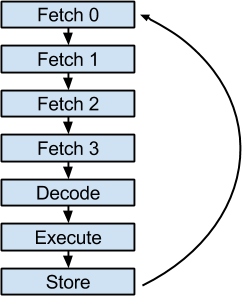
\includegraphics[width=0.5\linewidth]{./instruction_cycle.png}
                \caption{CPU Instruction Cycle}
            \end{minipage}
        \end{figure}

        Each instruction is 4 bytes long which requires 4 fetch stages
        to form the complete instruction word as our RAM only accesses
        single bytes at a time.  Typically, the next stage would be to
        decode the instruction as in some instruction sets the operands
        might cross byte boundaries and you need to wait until you have
        fetched all the bytes before you can decode the instruction. To
        simplify things, in our CPU the opcode and each operand get
        their own separate byte with the exception of memory addresses
        which require two bytes.  The side effect of this is that each
        operand can address up to 256 registers which in practice is
        unusual (a typical CPU might only have a couple dozen registers
        at most). We will consider this huge register file a feature as
        it actually makes writing a high level language compiler
        significantly easier as you do not need to worry about high
        pressure register allocation.  Since we do not actually have to
        decode the instruction the decode stage is used to increment
        the program counter and switch the memory address that the CPU
        is looking at to the address specified by the instruction.

        \vspace{\baselineskip}
        The table below summarizes the 22 instructions that are currently
        implemented.

        \begin{table}[H]
            \resizebox{\textwidth}{!}{%
            \centering
            \begin{tabular}{lllc}
                \toprule
                \textbf{Mnemonic} & \textbf{Operands} & \textbf{Description} & \specialcell{32-Bit Instruction Word\\MSb \hspace{1.75in} LSb}\\
                \midrule
                HALT &                 & Stop program execution                                         & \texttt{00000000 -------- -------- --------} \\
                LD   & \texttt{d,m} & Load value at address \texttt{m} into register \texttt{d}         & \texttt{00000001 dddddddd mmmmmmmm mmmmmmmm} \\
                ST   & \texttt{s,m} & Store register \texttt{s} into memory address \texttt{m}          & \texttt{00000010 ssssssss mmmmmmmm mmmmmmmm} \\
                STL  & \texttt{l,m} & Load literal \texttt{l} into memory address \texttt{m}            & \texttt{00000011 llllllll mmmmmmmm mmmmmmmm} \\
                LDL  & \texttt{d,l}    & Load literal \texttt{l} into register \texttt{d}               & \texttt{00000100 dddddddd aaaaaaaa --------} \\
                MOV  & \texttt{d,s}    & Move register \texttt{s} into register \texttt{d}              & \texttt{00000101 dddddddd aaaaaaaa --------} \\
                ADD  & \texttt{d,a,b}  & \texttt{d = a + b}                                             & \texttt{00000110 dddddddd aaaaaaaa bbbbbbbb} \\
                SUB  & \texttt{d,a,b}  & \texttt{d = a - b}                                             & \texttt{00000111 dddddddd aaaaaaaa bbbbbbbb} \\
                AND  & \texttt{d,a,b}  & \texttt{d = a \& b}                                            & \texttt{00001000 dddddddd aaaaaaaa bbbbbbbb} \\
                OR   & \texttt{d,a,b}  & \texttt{d = a | b}                                             & \texttt{00001001 dddddddd aaaaaaaa bbbbbbbb} \\
                XOR  & \texttt{d,a,b}  & \texttt{d = a $\oplus$ b}                                      & \texttt{00001010 dddddddd aaaaaaaa bbbbbbbb} \\
                SFL  & \texttt{d,a,b}  & \texttt{d = a << b}                                            & \texttt{00001011 dddddddd aaaaaaaa bbbbbbbb} \\
                SFR  & \texttt{d,a,b}  & \texttt{d = a << b}                                            & \texttt{00001100 dddddddd aaaaaaaa bbbbbbbb} \\
                INC  & \texttt{d,a,b}  & \texttt{d = a + 1}                                             & \texttt{00001101 dddddddd aaaaaaaa bbbbbbbb} \\
                DEC  & \texttt{d,a,b}  & \texttt{d = a - 1}                                             & \texttt{00001110 dddddddd aaaaaaaa bbbbbbbb} \\
                EQL  & \texttt{d,a,b}  & \texttt{d = a == b}                                            & \texttt{00001111 dddddddd aaaaaaaa bbbbbbbb} \\
                GTH  & \texttt{d,a,b}  & \texttt{d = a > b}                                             & \texttt{00010000 dddddddd aaaaaaaa bbbbbbbb} \\
                LTH  & \texttt{d,a,b}  & \texttt{d = a < b}                                             & \texttt{00010001 dddddddd aaaaaaaa bbbbbbbb} \\
                INV  & \texttt{d,a}    & \texttt{d = \texttildelow a}                                   & \texttt{00010010 dddddddd aaaaaaaa --------} \\
                BRZ  & \texttt{a,m} & Branch to \texttt{m} if register \texttt{a} is zero               & \texttt{00010011 aaaaaaaa mmmmmmmm mmmmmmmm} \\
                BRNZ & \texttt{a,m} & Branch to \texttt{m} if register \texttt{a} is not zero           & \texttt{00010100 aaaaaaaa mmmmmmmm mmmmmmmm} \\
                JMP  & \texttt{m}   & Jump to address \texttt{m}                                        & \texttt{00010101 mmmmmmmm mmmmmmmm --------} \\
                \bottomrule
        \end{tabular}}
            \caption{Instruction Set Description \& Encoding}
        \end{table}

    \subsection{Memory Mapping}

        \newcommand{\memsection}[4]{
            \bytefieldsetup{bitheight=#3\baselineskip}  % define the height of the memsection
            \bitbox[]{8}{
                \texttt{0x\uppercase{#1}}    % print end address
                \\ \vspace{#3\baselineskip} \vspace{-2\baselineskip} \vspace{-#3pt} % do some spacing
                \texttt{0x\uppercase{#2}} % print start address
            }
            \bitbox{16}{#4} % print box with caption
        }

        \newcommand{\memsectionone}[4]{
            \bytefieldsetup{bitheight=#3\baselineskip}  % define the height of the memsection
            \bitbox[]{8}{
                \texttt{0x\uppercase{#1}}    % print end address
                %\\ \vspace{#3\baselineskip} \vspace{-2\baselineskip} \vspace{-#3pt} % do some spacing
                %\texttt{0x\uppercase{#2}} % print start address
            }
            \bitbox{16}{#4} % print box with caption
        }

        \begin{figure}[H]
            \centering
            \begin{minipage}[t]{.5\textwidth}
                \vspace{0pt}
                All input, outputs, and internal peripherals such as the 32-bit
                timer and the UART are accessed and controlled via memory
                accesses in a scheme called memory-mapped IO \cite{io}. In this
                scheme each peripheral is assigned a memory address and then
                watches for this address on the memory bus. When the CPU writes
                to this address it stores the data to its own internal
                registers. When the CPU is doing a read we need a single entity
                in charge of figuring out which peripherals data to give to the
                CPU. This entity is called the memory mapper and it has a list
                of the memory addresses of all the peripherals. All the
                peripherals feed their outputs into the memory mapper.  The
                memory mapper then looks at the address that the CPU wants and
                feeds it the corresponding peripherals data. If the requested
                address does not belong to any peripheral the memory mapper
                selects the RAM as the CPU input.

                \vspace{\baselineskip}
                One downside of this approach is that we are wasting RAM. When
                the CPU writes to the memory address belonging to a peripheral
                that data also gets written into RAM but when the CPU reads
                back the memory at that address the memory mapper will direct
                the peripherals output to the CPU, not the RAMs output. In our
                case we have only a handful of memory mapped peripherals and
                lots of RAM so its not a huge deal.
            \end{minipage}%
            \begin{minipage}[t]{.5\textwidth}
                \vspace{0pt}
                \centering
                \begin{bytefield}{24}
                    \memsection{FFFF}{0020}{15}{Program Space}\\
                    \memsection{0019}{0013}{2}{Reserved}\\
                    \memsectionone{0012}{0012}{1}{UART Control / Status}\\
                    \memsectionone{0011}{0011}{1}{UART TX Data}\\
                    \memsectionone{0010}{0010}{1}{UART RX Data}\\
                    \memsection{000F}{0008}{2}{General Purpose Outputs}\\
                    \memsection{0007}{0000}{2}{General Purpose Inputs}\\
                \end{bytefield}
                \caption{SoC Memory Map}
            \end{minipage}
        \end{figure}

        The diagram to the right shows the memory map of our address space.
        There are 8 GPIs and 8GPOs and each one takes 1 byte.  The UART uses 3
        bytes, 2 for data in and out and a third one for status and control.
        Addresses \texttt{0x0013} through \texttt{0x0019} are reserved for
        future peripherals that might be added. The program space starts at
        \texttt{0x0020} and extends all the way to \texttt{0xFFFF} which gives
        the program about 65KB of usable space (not accounting for the size of
        the program itself). Note that this is the maximum amount of memory
        that the CPU is capable of addressing, it does not mean that amount of
        RAM will actually be available. The amount of RAM in FPGAs varies so
        the size of the RAM is configurable at build time by setting the
        \texttt{RAM\_ADDR\_BITS} define in the \texttt{constants.v} file. In my
        case, I can only fit about 8KB of RAM in the Cyclone II that is on my
        development board. Most actual production SoCs contain internal RAM but
        since I am targeting FPGAs, which might not have a lot of internal RAM,
        I did not want to make internal RAM a hard requirement so I brought out
        the RAM interface.  This makes it easy to use this project with
        external RAMs, such as the SRAM that is on my DE-1 development board.

    \subsection{Bootloader}

        \begin{figure}[H]
            \centering
            \begin{minipage}[t]{.6\textwidth}
                \vspace{0pt}
                One of the bigger challenges of running our system on an FPGA
                is loading the program into RAM.  Under simulation its as easy
                as using the \texttt{\$readmemb("filename")} but its not as
                straight forward when targeting a physical device. It is
                possible to bake the program in with the FPGA bitstream using a
                memory initialization file \cite{mif} but this would require us
                to resynthesize and flash the FPGA every time we wanted to run
                a new program.

                \vspace{\baselineskip}
                Another obvious solution would be to store the program on an SD
                card and write a hardware state machine to read it. While this
                initially seems like an attractive solution due to the ubiquity
                of SD cards it has three major drawbacks: interfacing with an
                SD card is not simple, not all FPGA development boards have an
                SD card slot, and every time you want to update the program you
                have to remove the SD card, put it in your computer, change the
                program, take it out, put it back in the dev board, and reset
                the FPGA.  For rapid development, which is what we want to do,
                this process is unacceptable.

                \vspace{\baselineskip}
                Yet another solution is to load our
                program via a serial port. All FPGAs are capable of
                implementing a UART and getting a USB to UART adaptor is cheap
                and easy. Also, with this method we can simply press a button
                on the development board to put the system into `boot mode' and
                then run a little script on the computer to send over program.
                The only disadvantage of this method is that the program is
                volatile, if we power cycle the board we have to resend the
                program. Since the goals of this project do not involve
                embedding our FPGA into a system that needs to be able to
                survive power cycles the UART solution is great.
            \end{minipage}%
            \begin{minipage}[t]{.4\textwidth}
                \vspace{0pt}
                \centering
                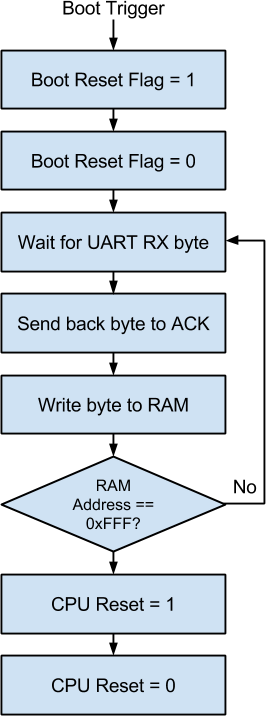
\includegraphics[width=0.65\linewidth]{./bootloader.png}
                \caption{Bootloader State Machine}
            \end{minipage}
        \end{figure}

        The UART bootloader needs to be able to do 2 main things: receive and
        write a program to RAM, and reset the CPU after its done. The state
        diagram shown to the right illustrates this process. The state machine
        sits in an idle state until a boot trigger event, which in the case of
        this project is just a button press. It then drops through two states
        which pulse the boot reset flag. This flag is used to reset the UART to
        clear any status flags that may be set. The bootloader also asserts a
        signal to indicate that it is in boot mode. This switches the RAMs
        address and data lines from the CPU to the bootloader. The bootloader
        then continuously reads bytes from the UART and loads them into RAM,
        incrementing the RAM address after each byte, until it reaches the top
        of the RAM. The disadvantage of this method is that we have to send the
        full RAM contents, even if it is mostly zeros. This is significantly
        slower than just sending the RAM contents that the program actually
        occupies.  A possible solution to this might be to run length encode
        the data but with small RAM sizes (like the one in our system) it only
        takes a few seconds to load so the effort of speeding it up is probably
        not worth it. Once the bootloader has determined that it has received
        all the bytes it puts the CPU in reset and de-asserts the boot mode
        flag. It then de-asserts the CPU reset line and execution begins. It is
        important to have the CPU in reset before de-asserting the boot mode
        flag as once the flag is de-asserted the CPU has control over the RAM.
        Since the contents of RAM were unknown and changing during boot the CPU
        could be executing anywhere. We don't want to give control of the RAM
        back to the CPU until we reset it.


    \newpage
    \subsection{Assembler}

    To construct a program that can run on our CPU we simply need to lookup the
    binary encoding of the instruction that we want to use. While it is
    certainly possible to assemble a program by hand its much less tedious to
    have an assembler do it for you. I have created a simple assembler
    (\texttt{./tools/asm.py}) which supports some of the typical features one
    would expect from an assembler.

    The assembler reads the input \texttt{.asm} file line by line and first
    strips the line of comments and forces it to upper case. It then figures
    out if the line is a directive (like \texttt{.define}), an instruction, or
    a label. If it is an instruction it forms the 4 byte instruction word
    (using the OP code that it automatically parses out of the Verilog
    \texttt{constants.v} file) and adds those bytes to an array. If it comes
    across a label it records the name of the label and what byte location it
    is at. When it comes across a jump it records what the destination label is
    and then just fills in zeros for the address since it might not know what
    the address of the label is yet (if it wants to jump forward in the program
    we do not yet know the address of that label).  After all instruction bytes
    have been added to the array it goes back through all the jumps, looks up
    the position of the label it wants to jump to, and fills out the address of
    the jump instruction. It then writes all the bytes out to two files: one
    file which is a raw binary file that we will load into the FPGA, and
    another which is an ASCII file formatted in a way that can be read in by
    the Verilog simulator.

    Other features such as aliases, the equivalent to \texttt{\#define} in C,
    are supported through the \texttt{.define} directive and comments are fully
    supported as well. The assembler also parses the \texttt{constants.v} file
    to figure out the memory location of all the memory mapped peripherals and
    automatically adds an alias for them. This is nice since when you add a new
    peripheral you only have to update the Verilog file and the assembler
    automatically will account for it. The whole assembler is only about 150
    lines of code, most of which is just putting the operands in the correct
    byte order for each instruction.

    An example program which increments the value shown on the  LEDs every time
    the timer goes off is shown below.

    \lstinputlisting[caption=Count up on the LEDs]{../tools/count.asm}


\newpage
\section{Results}

    The results of this project are best conveyed through video. The following
    videos show the CPU running four different test programs on the DE-1
    development board.

    \begin{table}[H]
        \centering
        \begin{tabular}{lll}
            \toprule
            \textbf{Test Program} & \textbf{Description} & \textbf{Video Link} \\
            \midrule
            \texttt{shift.asm}      & Shifts a single LED down both sets of LEDS     & \url{http://youtu.be/aNCSzHn3NVQ} \\
            \texttt{count.asm}      & Counts up in binary on the LEDs                & \url{http://youtu.be/9p6P2v8b_BA} \\
            \texttt{seg\_count.asm} & Counts up in base 10 on the 7-segment displays & \url{http://youtu.be/zjMZnJXbdMo} \\
            \texttt{blink\_1hz.asm} & Blinks the green LEDs at 1hz                   & \url{http://youtu.be/qbEIPBlEjM4} \\
            \bottomrule
        \end{tabular}
    \end{table}

    We can see from the videos above that the CPU and supporting components all
    seem to be working as expected. While these small test programs are no
    where near what a typical application might be like it at least proves that
    the system is working at a fundamental level and that all of our
    development tools are working correctly. With just 2 lines of Verilog and 4
    lines of Python we can add additional instructions to the CPU and start
    exploring more complex topics and designs in the future. Given the ease in
    which we can modify and extend this project I belive we have achieved the
    original goal of building a complete example system from the CPU all the
    way to the compiler.

\section{Discussion}

\newpage
\begin{thebibliography}{9}

    % \cite{gg}
    %\bibitem{gg} \url{http://mo5.com/musee-machines-gamegear.html}
    \bibitem{yfcpu} \url{http://colinmackenzie.net/index.php?option=com_content&view=article&id=11:your-first-cpu&catid=8:rotator&Itemid=7}
    \bibitem{flex} \url{http://aquamentus.com/flex_bison.html}
    \bibitem{cycle} \url{http://en.wikipedia.org/wiki/Instruction_cycle}
    \bibitem{von} \url{http://en.wikipedia.org/wiki/Von_Neumann_architecture}
    \bibitem{modify} \url{http://en.wikipedia.org/wiki/Self-modifying_code}
    \bibitem{harvard} \url{http://en.wikipedia.org/wiki/Harvard_architecture}
    \bibitem{io} \url{http://en.wikipedia.org/wiki/Memory-mapped_I/O}
    \bibitem{mif} \url{http://quartushelp.altera.com/13.0/mergedProjects/reference/glossary/def_mif.htm}
\end{thebibliography}

\end{document}

\subsection{Placement}

    \subsubsection{Placement Grid Dimensions}

        One of the main goals of this project is to have a final layout that is
        as close to a perfect square as possible. We call this the
        \texttt{squareness} of our layout which is the ratio of width to height (
        \texttt{squareness = width / height}).  The closer this value is to 1
        the `more square' the layout is.  The main issue with achieving this is
        that we do not know up front how tall our layout will end up since the
        channels between the cells are variable and the width and height of the grid
        directly effect them.

        In order to figure out what width and height we should make our grid we need
        to come up with some heuristic that can estimate the squareness of a layout
        given only the placement grid dimensions, number of cell, and number of nets.

        \begin{figure}[H] \centering
            \includegraphics{./square_f.png}
            \caption{Squareness Function}
        \end{figure}

        Once we have an equation that can estimate the squareness we can plug
        in different grid dimensions and figure out one that gets us the best
        squareness. In order to figure out the formula that estimates our
        squareness we manually specified various grid dimensions for each
        benchmark and recorded the resulting squareness. This data can be found
        in the Appendix section at the end of the report. We then used the
        program Eureqa to evolve an equation that fit our data. After running
        Eureqa for 15 minutes we had an equation that fit our data with an $
        R^{2} =  0.9965 $.

        \begin{figure}[H]
            \centering
            \includegraphics[width=\linewidth]{./square_eq.png}
            \caption{Squareness Equation}
        \end{figure}

        To calculate the placement grid size we start the grid as a perfect
        square by taking the square root of the number of cells. We then
        decrease the height and increase the width and check the squareness of
        this size. We continue doing this and keeping track of which size
        results in the best squareness until the height is 0.

        The table below shows the resulting squareness of the original method
        (just making a perfectly square grid) versus using the equation. We
        can see that by using the equation we achieved a much more square
        layout for all but benchmark 9. This could be a result of not having
        enough data points to fit a better curve with.

        \begin{table}[H]
            \centering
            \begin{tabular}{c|ccc|ccc|c}
                \toprule
                & \multicolumn{3}{c}{\specialcell{Without Equation}} & \multicolumn{3}{|c|}{\specialcell{With Equation}} & \\
                \textbf{Benchmark} &
                \specialcell{Grid\\Width} & \specialcell{Grid\\Height} & \specialcell{Layout\\Squareness} &
                \specialcell{Grid\\Width} & \specialcell{Grid\\Height} & \specialcell{Layout\\Squareness} &
                \specialcell{Percent\\Improvement} \\
                \midrule
                 1  & \phantom{0}7 & \phantom{0}7 & 0.7245 & \phantom{0}9 & \phantom{0}5 & 1.0789 &           19.66 \% \\
                 2  &           10 & \phantom{0}9 & 0.7365 &           12 & \phantom{0}8 & 0.9845 &           24.80 \% \\
                 3  &           14 &           13 & 0.6767 &           18 &           10 & 1.0914 &           23.18 \% \\
                 4  &           19 &           19 & 0.7029 &           28 &           13 & 1.2579 & \phantom{0}3.92 \% \\
                 5  &           27 &           27 & 0.6125 &           45 &           16 & 1.2060 &           18.16 \% \\
                 6  &           32 &           32 & 0.6060 &           56 &           18 & 1.1735 &           22.05 \% \\
                 7  &           23 &           22 & 0.6452 &           39 &           13 & 0.9823 &           33.71 \% \\
                 8  &           30 &           30 & 0.6306 &           50 &           18 & 1.3123 & \phantom{0}5.70 \% \\
                 9  &           29 &           28 & 0.6343 &           45 &           18 & 1.4323 &           -6.67 \% \\
                 10 &           25 &           24 & 0.6715 &           36 &           17 & 1.2772 & \phantom{0}5.13 \% \\
                \bottomrule
            \end{tabular}
            \caption{Improvement from using squareness estimate equation}
        \end{table}

        \newpage
        \subsubsection{Force Directed Placement}

        We use a force directed placement algorithm in order to reduce the
        overall complexity. Our algorithm follows the one in the book exactly
        with the exception of what happens when the target cell is locked. In
        the original algorithm you search for a vacant spot to place the seed
        cell if the target cell is locked, we expand that to also include
        unlocked spots. If we choose an unlocked spot then that cell we are
        replacing becomes the new seed cell.  We found through experimentation
        that this achieves less complex placements. The gray cells are cells
        with no connections.

        \begin{figure}[H]
            \centering
            \includegraphics[width=\linewidth, height=2in, keepaspectratio]{../benchmarks/10_placement_0_start.jpg}
            \caption{Original}
        \end{figure}
        \begin{figure}[H]
            \centering
            \includegraphics[width=\linewidth, height=2in, keepaspectratio]{../benchmarks/10_placement_1_force.jpg}
            \caption{Force Directed}
        \end{figure}

        In order to figure out the best abort limit we recorded the layout area
        for each benchmark for various limits. We found the abort limit that
        achieved the minimum area and used that minimum area to normalize the
        areas of the others as a percent increase. We found that an abort limit
        of 1 gives us the lowest average percent increase in area across all
        the benchmarks.

        \begin{figure}[H]
            \centering
            \begin{minipage}{.5\textwidth}
                \centering
                \includegraphics[width=0.98\linewidth]{./abort_limit.png}
            \end{minipage}%
            \begin{minipage}{.5\textwidth}
                \centering
                \includegraphics[width=0.98\linewidth]{./abort_limit_stacked.png}
            \end{minipage}
            \caption{Percent increase in layout area versus abort limit}
        \end{figure}

        \subsubsection{Flipping Cells}

        The force directed algorithm does not take into account the positions
        of the terminals on each cell, it assumes all connections go to the
        center of the cell. This results in a lot of connections that
        unnecessarily span vertically across a row. To fix these we simply go
        through each cell and try all possible flip orientations and see which
        one reduces the wirelength the most. This approach is not ideal as it
        does not take into consideration chains of cells that all may need to
        be flipped. An approach similar to KL where we walk down the connection
        tree trying flips and only actually flip as many as what improves
        the total wirelength would be interesting. Unfortunately we did not
        have time to explore this.

        \begin{figure}[H]
            \centering
            \includegraphics[width=\linewidth, height=4in, keepaspectratio]{../benchmarks/10_placement_1_force.jpg}
            \caption{Original}
        \end{figure}
        \begin{figure}[H]
            \centering
            \includegraphics[width=\linewidth, height=4in, keepaspectratio]{../benchmarks/10_placement_2_flip.jpg}
            \caption{Flipped}
        \end{figure}

        \subsubsection{Adding Feed-Through Cells}

        In order to channel route we cannot have connections that span rows. To
        fix this we add feed-through cells (shown in light gray) in order to
        transfer the nets between rows. The process of adding feed-through cells
        starts at the bottom row. It goes through each terminal of each cell
        and detects if the terminal is in the same channel as its destination
        terminal. If it's not, it figures out if it needs to add a feed-through
        to the current row (say the terminal is at the bottom of the cell and
        it needs to connect to somewhere above it) or if it needs to add the
        feed-through to the next row up (if the terminal is at the top of the
        cell but it connects to the top of the cell above it). If a feed-through
        cell is added the whole row is rescanned since we might need to
        add yet another feed-through cell for the feed-through we just placed.

        \begin{figure}[H]
            \centering
            \includegraphics[width=\linewidth, height=4in, keepaspectratio]{../benchmarks/10_placement_2_flip.jpg}
            \caption{Original}
        \end{figure}
        \begin{figure}[H]
            \centering
            \includegraphics[width=\linewidth, height=4in, keepaspectratio]{../benchmarks/10_placement_3_feed.jpg}
            \caption{With feed-throughs}
        \end{figure}

        \subsubsection{Evening Row Lengths}

        After adding the feed-through cells the row lengths become uneven. In
        order to fix this we add all unconnected cells to a queue and then go
        through them adding them to which ever row is currently the shortest.
        Additionally, we alternate placing them on either side and we also skip
        every other cell. The reason behind this is that since we just messed
        up a lot of the force directed work by removing all the unconnected
        cells we will have to re-force direct them within their rows. Spacing
        them out will allow them to more easily move around and have a higher
        chance of finding a vacant spot close to their target.

        \begin{figure}[H]
            \centering
            \includegraphics[width=\linewidth, height=4in, keepaspectratio]{../benchmarks/10_placement_3_feed.jpg}
            \caption{Original}
        \end{figure}
        \begin{figure}[H]
            \centering
            \includegraphics[width=\linewidth, height=4in, keepaspectratio]{../benchmarks/10_placement_4_feed_even.jpg}
            \caption{Even length rows}
        \end{figure}

        \subsubsection{Pulling Cells Closer}

        After evening out the row lengths we are left with a lot of space
        between connected cells. In order to fix this we run a simplified force
        directed algorithm which goes through each cell, calculates its zero
        force location on the x axis, and then finds the closest unconnected
        cell to that location and swaps its position with it.

        \begin{figure}[H]
            \centering
            \includegraphics[width=\linewidth, height=4in, keepaspectratio]{../benchmarks/10_placement_4_feed_even.jpg}
            \caption{Original}
        \end{figure}
        \begin{figure}[H]
            \centering
            \includegraphics[width=\linewidth, height=4in, keepaspectratio]{../benchmarks/10_placement_5_pull.jpg}
            \caption{Cells pulled closer}
        \end{figure}

        \newpage
        \subsubsection{Moving Feed-Through Cells}

        Sometimes, because it can not be know at the time of placement, the
        feed-through cells end up on the far side of the cell as shown in the
        `before' picture. We make an effect to detect these and move them
        closer.  We always want the feed-through cell to horizontally between
        the two terminals it is connected to. (This is done before routing
        begins, the example images below show the circuit post routing as it
        better illustrates the situation)

        \begin{figure}[H]
            \centering
            \begin{minipage}{.5\textwidth}
                \centering
                \includegraphics[width=0.7\linewidth]{./move_ft_before.png}
                \caption{Before}
            \end{minipage}%
            \begin{minipage}{.5\textwidth}
                \centering
                \includegraphics[width=0.7\linewidth]{./move_ft_after.png}
                \caption{After}
            \end{minipage}
        \end{figure}


\newpage
\subsection{Routing}

    \subsubsection{Assigning nets to track}

        Routing begins by first assigning each net to its own track. Net
        collisions are not considered at this point.

        \begin{figure}[H]
            \centering
            \includegraphics[width=\linewidth]{./route_0_crop.png}
            \caption{Each net has its own track}
        \end{figure}

    \subsubsection{Expand the tracks}

        Each net is checked to see if it conflicts with another net. Some
        conflict configurations can be solved by adding another track to the
        channel (expanding the channel). The image below shows the same circuit
        at the previous image but with the conflict now solved and circled in
        red.

        \begin{figure}[H]
            \centering
            \includegraphics[width=\linewidth]{./route_1_crop.png}
            \caption{Conflict is solved by expanding the channel}
        \end{figure}

    \subsubsection{Fixing overlaps}

        Some conflicts are true overlaps that cannot be solved no matter what
        net ordering you try. The only way to solve these conflicts is to move
        the cells in the rows over. The image on the left shows an overlap
        between nets 11 and 29. The only way to solve this is to move cell C36
        over to the right, which is shown in the image on the right.

        \begin{figure}[H]
            \centering
            \begin{minipage}{.5\textwidth}
                \centering
                \includegraphics[width=0.75\linewidth]{./route_1_overlap.png}
                \caption{Overlapping nets}
            \end{minipage}%
            \begin{minipage}{.5\textwidth}
                \centering
                \includegraphics[width=0.75\linewidth]{./route_2_crop.png}
                \caption{Conflict is solved by moving cells over}
            \end{minipage}
        \end{figure}

    \subsubsection{Finding Vertical Nets}

        For terminals that line up directly with their destination we can use a
        purely vertical net that doesn't take up a track. The image on the left
        shows a small horizontal segment that is currently occupying a track.
        We simply mark this net as purely vertical and remove it from any
        future track related operations.

        \begin{figure}[H]
            \centering
            \begin{minipage}{.5\textwidth}
                \centering
                \includegraphics[height=3in]{./route_2_vertical.png}
                \caption{Vertical net taking up a track}
            \end{minipage}%
            \begin{minipage}{.5\textwidth}
                \centering
                \includegraphics[height=3in]{./route_3_crop.png}
                \caption{Unnecessary horizontal segment removed}
            \end{minipage}
        \end{figure}

    \subsubsection{Pulling Nets Up}

        We next want to try to shrink the channel so the first step is to pull
        all the nets either up or down. Nets are pulled up as far as possible
        without causing a conflict.  We do not consider any specific ordering
        about which nets we pull up first although it can effect the final
        configuration. The image below shows the result of pulling all the nets
        up and then removing tracks which not longer have any nets on it.

        \begin{figure}[H]
            \centering
            \includegraphics[width=\linewidth]{./route_4_crop.png}
            \caption{All nets pulled up and empty tracks removed}
        \end{figure}

    \subsubsection{Pulling Nets In}

        For nets whos terminals are both on the same side of the channel we
        want to bring that net back to that side (pull it in to the side the
        terminals are on). The image below shows the result of doing that.

        \begin{figure}[H]
            \centering
            \includegraphics[width=\linewidth]{./route_5_crop.png}
            \caption{Nets pulled in closest to the cells the connect to}
        \end{figure}

        In our actual implementation we pull the cells up, then in, then down,
        then in again. This routine seems to be able to achieve fairly high
        channel density.

\newpage
\section{Usage}

Building is accomplished via a \texttt{Makefile} which generates an executable
names \texttt{main}.  Additional build opions are shown below.

\begin{lstlisting}[language=bash]
$ make              # regular build
$ make clang        # builds using clang++ instead of g++
$ make debug        # enable debug printfs
$ make clean        # removes all binaries, object files, and benchmark results
$ make benchmarks   # runs all the benchmarks in the 'benchmark' directory
$ make pngs         # converts all the benchmark .svg files to .png
$ make jpgs         # converts all the .png files to reduced resolution .jpg files
\end{lstlisting}

The program accepts a single argument which is a file containing the netlist
formatted as specified in the assignment. All log and debug output is printed
to \texttt{stdout} and the output .mag and .svg files are named the same as the
input file.

\begin{lstlisting}[language=bash]
$ ./main benchmark/1 > benchmark/1.log
$ ls benchmark/1.*
benchmarks/1.log  benchmarks/1.mag benchmarks/1.svg
\end{lstlisting}

\section{Results}

    The results of all the benchmark netlists are tabulated below. The
    wirelength is the length post routing.

    \begin{table}[H]
        \centering
        \begin{tabular}{ccccccccc}
            \toprule
            \textbf{Benchmark} &
            \specialcell{Box X} & \specialcell{Box Y} & \specialcell{Box Area} &
            \specialcell{\# FTs} & \specialcell{Wirelength} & \specialcell{\# Vias} &
            \specialcell{Execution Time} & \specialcell{Memory Usage}\\
            \midrule
            \phantom{0}1 & \phantom{00}82 & \phantom{00}76 & \phantom{000}6232 & \phantom{00}17 & \phantom{00}1093 & \phantom{0}112 & 0.009873s & \phantom{0}296 kB \\
            \phantom{0}2 & \phantom{0}127 & \phantom{0}129 & \phantom{00}16383 & \phantom{00}50 & \phantom{00}2547 & \phantom{0}270 & 0.021806s & \phantom{0}340 kB \\
            \phantom{0}3 & \phantom{0}191 & \phantom{0}175 & \phantom{00}33425 & \phantom{0}112 & \phantom{00}6114 & \phantom{0}562 & 0.044696s & \phantom{0}424 kB \\
            \phantom{0}4 & \phantom{0}317 & \phantom{0}252 & \phantom{00}79884 & \phantom{0}213 & \phantom{0}14108 & \phantom{}1126 & 0.111609s & \phantom{0}588 kB \\
            \phantom{0}5 & \phantom{0}486 & \phantom{0}403 & \phantom{0}195858 & \phantom{0}464 & \phantom{0}41469 & \phantom{}2336 & 0.384445s & \phantom{0}916 kB \\
            \phantom{0}6 & \phantom{0}602 & \phantom{0}513 & \phantom{0}308826 & \phantom{0}685 & \phantom{0}70536 & \phantom{}3322 & 0.670760s & \phantom{}1204 kB \\
            \phantom{0}7 & \phantom{}1110 & \phantom{}1130 & \phantom{}1254300 & \phantom{}1738 & \phantom{}443767 & \phantom{}5448 & 1.581445s & \phantom{}1512 kB \\
            \phantom{0}8 & \phantom{0}437 & \phantom{0}333 & \phantom{0}145521 & \phantom{0}297 & \phantom{0}22907 & \phantom{}1994 & 0.360278s & \phantom{0}912 kB \\
            \phantom{0}9 & \phantom{0}328 & \phantom{0}229 & \phantom{00}75112 & \phantom{00}69 & \phantom{00}6097 & \phantom{0}842 & 0.206668s & \phantom{0}664 kB \\
            \phantom{}10 & \phantom{0}258 & \phantom{0}202 & \phantom{00}52116 & \phantom{00}35 & \phantom{00}2881 & \phantom{0}404 & 0.157362s & \phantom{0}544 kB \\
            \bottomrule
        \end{tabular}
        \caption{Result Summary}
    \end{table}

\foreach \i in {1,...,10} {
    \newpage
    \subsection{Benchmark \i\thinspace - Placement Steps}
    \placementimage{../benchmarks/\i_placement_0_start.jpg}      {Benchmark \i\thinspace - Step 1/7 - Initial placement}
    \placementimage{../benchmarks/\i_placement_1_force.jpg}      {Benchmark \i\thinspace - Step 2/7 - Force directed placement}
    \placementimage{../benchmarks/\i_placement_2_flip.jpg}       {Benchmark \i\thinspace - Step 3/7 - Flip cells}
    \placementimage{../benchmarks/\i_placement_3_feed.jpg}       {Benchmark \i\thinspace - Step 4/7 - Add feed-throughs}
    \placementimage{../benchmarks/\i_placement_4_feed_even.jpg}  {Benchmark \i\thinspace - Step 5/7 - Even out the row length}
    \placementimage{../benchmarks/\i_placement_5_pull.jpg}       {Benchmark \i\thinspace - Step 6/7 - Pull cells in the rows closer together}
    \placementimage{../benchmarks/\i_placement_6_feed_moved.jpg} {Benchmark \i\thinspace - Step 7/7 - Move feed-throughs to optimal location}

    \newpage
    \subsection{Benchmark \i\thinspace - Final Routing}
    \begin{figure}[H]
        \centering
        \includegraphics[width=\linewidth]{../benchmarks/\i.jpg}
        \caption{Benchmark \i\thinspace - Final routing}
    \end{figure}

    \newpage
    \subsection{Benchmark \i\thinspace - Magic Screenshot}
    \begin{figure}[H]
        \centering
        \includegraphics[width=\linewidth]{./magic_\i.png}
        \caption{Benchmark \i\thinspace - Magic Screenshot}
    \end{figure}

    \newpage
    \subsection{Benchmark \i\thinspace - Log file}
    \lstinputlisting[caption=Benchmark \i\thinspace - Log]{../benchmarks/\i.log}
}

\newpage
\section{Retrospective}

Overall, we are pretty satisfied with both the execution speed and quality of
our results. All of our execution times with the exception of benchmark 7 are
under half a second. We also feel that our memory usage is minimal as we only
store one vector of actual cell objects and all other data structures just
contain pointers back to the original objects. We also make heavy use of pass
by reference to avoid needlessly copying big data structures into functions.

In terms of placement and routing quality there is always room for improvement.
It's easy to visually look at almost any result and see ways that it could be
improved but how to translate these improvements into algorithms is not always
so obvious. We believe, however, that we were are able to handle a lot of
specific cases (like moving the feed-throughs to the other side of the cell)
which in the end resulted in superior layouts.  For the force directed
placement algorithm it is hard to tell if the results you get are truly the
best, especially when the circuit is so large you cannot visually comprehend
it. We feel like we did our best analyzing it empirically and tuned is to best
suit our benchmark files. One of the main problems with the force directed
algorithm is that it tends to pull all the cells into the center of the layout.
We tried to fix this by redistributing the unconnected cells evenly through the
layout and then re-force directing the rows but it is still not always ideal.
One interesting method to pursue would be using a combination of min-cut /
quadratic placement and then force directing the sub divisions (or vice versa).
If we were to min-cut horizontally we might be able to reduce some nets that
currently span multiple rows.


\newpage
\section{Appendix}

\begin{table}[H]
    \centering
    \begin{tabular}{cccccc}
        \toprule
        \textbf{Benchmark} & \textbf{Num Cells} & \textbf{Num Nets} & \textbf{Grid Width} & \textbf{Grid Height} & \textbf{Squareness}\\
        \midrule

        1  & 45   & 45   & 7  & 7  & 0.72449 \\
        2  & 90   & 90   & 10 & 9  & 0.736486 \\
        3  & 180  & 180  & 14 & 13 & 0.676724 \\
        4  & 360  & 360  & 19 & 19 & 0.702857 \\
        5  & 720  & 720  & 27 & 27 & 0.612457 \\
        6  & 1000 & 1000 & 32 & 32 & 0.605988 \\
        7  & 500  & 1000 & 23 & 22 & 0.645203 \\
        8  & 900  & 720  & 30 & 30 & 0.630648 \\
        9  & 800  & 360  & 29 & 28 & 0.634349 \\
        10 & 600  & 180  & 25 & 24 & 0.67148 \\
        \midrule

        1  & 45   & 45   & 8  & 6  & 0.820225 \\
        2  & 90   & 90   & 27 & 8  & 0.984496 \\
        3  & 180  & 180  & 12 & 12 & 0.755981 \\
        4  & 360  & 360  & 15 & 18 & 0.740413 \\
        5  & 720  & 720  & 20 & 26 & 0.595577 \\
        6  & 1000 & 1000 & 28 & 31 & 0.561298 \\
        7  & 500  & 1000 & 33 & 21 & 0.614935 \\
        8  & 900  & 720  & 24 & 29 & 0.637652 \\
        9  & 800  & 360  & 32 & 27 & 0.685294 \\
        10 & 600  & 180  & 30 & 23 & 0.75 \\
        \midrule

        1  & 45   & 45   & 9  & 5  & 1.078947 \\
        2  & 90   & 90   & 13 & 7  & 1.20339 \\
        3  & 180  & 180  & 17 & 11 & 0.921875 \\
        4  & 360  & 360  & 22 & 17 & 0.833333 \\
        5  & 720  & 720  & 29 & 25 & 0.681979 \\
        6  & 1000 & 1000 & 34 & 30 & 0.583232 \\
        7  & 500  & 1000 & 25 & 20 & 0.646465 \\
        8  & 900  & 720  & 33 & 28 & 0.672032 \\
        9  & 800  & 360  & 31 & 26 & 0.731629 \\
        10 & 600  & 180  & 28 & 22 & 0.773946 \\
        \midrule

        1  & 45   & 45   & 12 & 4  & 1.779661 \\
        2  & 90   & 90   & 15 & 6  & 1.623762 \\
        3  & 180  & 180  & 18 & 10 & 1.091429 \\
        4  & 360  & 360  & 23 & 16 & 0.84127 \\
        5  & 720  & 720  & 30 & 24 & 0.742911 \\
        6  & 1000 & 1000 & 35 & 29 & 0.624372 \\
        7  & 500  & 1000 & 27 & 19 & 0.692828 \\
        8  & 900  & 720  & 34 & 27 & 0.711864 \\
        9  & 800  & 360  & 32 & 25 & 0.790323 \\
        10 & 600  & 180  & 29 & 21 & 0.869748 \\
        \midrule

        1  & 45   & 45   & 15 & 3  & 2.923077 \\
        2  & 90   & 90   & 18 & 5  & 1.864583 \\
        3  & 180  & 180  & 20 & 9  & 1.322368 \\
        4  & 360  & 360  & 24 & 15 & 0.920382 \\
        5  & 720  & 720  & 32 & 23 & 0.75098 \\
        6  & 1000 & 1000 & 36 & 28 & 0.699068 \\
        7  & 500  & 1000 & 28 & 18 & 0.715323 \\
        8  & 900  & 720  & 35 & 26 & 0.694501 \\
        9  & 800  & 360  & 34 & 24 & 0.810289 \\
        10 & 600  & 180  & 30 & 20 & 0.991111 \\
        \midrule

        1  & 45   & 45   & 23 & 2  & 4.945946 \\
        2  & 90   & 90   & 23 & 4  & 2.626667 \\
        3  & 180  & 180  & 23 & 8  & 1.391608 \\
        4  & 360  & 360  & 26 & 14 & 0.986532 \\
        5  & 720  & 720  & 33 & 22 & 0.848671 \\
        6  & 1000 & 1000 & 38 & 27 & 0.674667 \\
        7  & 500  & 1000 & 30 & 17 & 0.763196 \\
        8  & 900  & 720  & 36 & 25 & 0.832599 \\
        9  & 800  & 360  & 35 & 23 & 0.883333 \\
        10 & 600  & 180  & 32 & 19 & 1.074074 \\

        \bottomrule
    \end{tabular}
    \caption{Squareness Trial Data}
\end{table}


\end{document}
